\chapter{Introduction}
\label{introductions}

\begin{abstract}
Gold nanorods are ideal candidates for complementing fluorophores in labelling
applications. The presence of the surface plasmon resonance generates large
absorption and scattering cross sections, thus making the detection of single
nanoparticles possible under a light microscope. In this introduction we will
review the current status of light microscopy, particularly of fluorescece
microscopes. We will introduce some properties of gold nanoparticles including
the plasmon resonance and we will focus into the luminescence emission.
Finally we will briefly introduce the experimental chapters of this
thesis, that correspond to applications of the luminescence ranging from imaging to
temperature sensing.
\end{abstract}

\newpage

\section{Light Microscopy}
\dropcap{M}{icroscopes} have become indispensable tools in material science and
biology. The first microscopes developed by Antoni Van Leeuwenhoek in the XVII
century were aimed at studying fabrics; it didn't take long however to discover
that nature was hiding amazing details beyond what the bare human eye could
see. The first microscope builders focused into developing better lenses in
order to obtain sharper images and therefore being able to observe even smaller
structures. 

With the development of the wave theory of light a fundamental limitation for
optical microscopes appeared: the diffraction limit. Abbe realized that no
matter how good a lens is, there will always be a limit to how much it is
possible to focus light. This limit is determined mainly by the wavelength of
the employed light beam and by the maximum acceptance angle of the lens.
Improving the optics is a technical challenge that however has a geometrical
limit. On the other hand, the wavelength of the sources is the parameter that
can be modified.

Shortening the irradiation wavelength would increase the resolution of a
microscope. Particles with wavelengths shorter than optical wavelengths, such as
electrons, opened the possibility to investigate much smaller
structures\cite{Kausche1939}. Notably in the field of virology the electron
microscope provided the evidence that researchers were long looking for: the
existence of particles smaller than what optical microscopes were able to
resolve. Electron microscopes are a very powerful tool but they require special
sample preparations that don't allow the study of biological processes
\textit{in vivo}.

With a similar strategy, the resolution of optical microscopes can be increased
with the use of ultraviolet sources. Some biological samples show emission of
light at longer wavelengths when irradiated with UV light, nowadays simply
referred to as autofluorescence. In $1911$ German physicist Oskar Heimst\"{a}dt
used the the emission from bacteria to build the first fluorescence
microscope\cite{Heimstadt1911}. The difficulties to focus enough UV light into
the sample and the low efficiency in collecting the emission made him skeptical
of the success of his design. He ended his work stating\cite{Rusk2009},

\begin{displayquote}
If and to what degree fluorescence microscopy will widen the possibilities of
microscopic imaging only the future will show.
\end{displayquote}

Fluorescence however was not a new phenomenon. It was first observed and
characterized during the second half of the $19$th century. The pioneering works
of Stokes showed that some materials when irradiated with short wavelengths emit
light at longer ones. It was only in the $1930$s when the first applications of
fluorescent materials started to emerge for biological applications.
Fluorophores were employed to stain biological samples, allowing to easily
detect tissue components or bacteria. Oskar Heimst\"{a}dt could rest assured
that his invention was starting to revolutionized biology. 

The following decades witnessed a phenomenal increase in technical developments,
including the advancement of epi-illimuniation, the confocal microscope and the
improvement of filters and light sources. The dichromatic mirror, the final key
element of a fluorescence microscope, was introduced in $1967$\cite{Ploem1967}.
The wealth of information that could be retrieved thanks to fluorescence and its
simple implementation were crucial for the success of the fluorescence
microscope and its establishment as a standard tool in almost any biological or
material science laboratory. Fluorescence microscopes however do not overcome
the diffraction limit. 

At the end of the XX century a major breakthrough occurred in the field of
optics: the detection of a single-molecule fluorescence in
$1990$\cite{PhysRevLett.65.2716}. Single-molecules opened the door to determine
material properties that would have been hidden by ensemble averaging.
The first studies were done at low temperature (few Kelvins) and gave access to
properties not only of the fluorescent molecules themselves but also of the
hosting matrices, mainly polymers and crystals. Single-molecules are the bridge
between the diffraction limit of far field optics and the atomic scale
properties of materials. 

Single molecule microscopy also changed the way imaging can be performed. If two
fluorophores are separated further away than the diffraction limit, their
centers can be determined with a precision that scales as $\approx 1/\sqrt{N}$,
with $N$ the number of recorded photons. The possibility of localizing single
molecules beyond Abbe's limit show how useful single molecule detection could
be. For example, tracking of single molecules\cite{Schmidt1996} could be used to
study diffusion with unprecedented spatial and temporal resolutions.

In relevant biological samples, however, the density of fluorophores is such
that they are not further apart than diffraction limit. In the late $1990$s it
was found that the fluorescence of molecules can be switched on and off by
irradiating them with specific wavelengths\cite{Moerner1997}. This led to the
development of a wide variety of techniques that rely on switching on and off
molecules\cite{Betzig2006} such that they can be individually
localized\cite{Dertinger2009}. Post processing the information of each
fluorescent molecule allows to reconstruct images with a spatial resolution an
order of magnitude higher than the diffraction limit\cite{Moerner2007}.

Molecules, however, show two phenomena known as blinking\cite{Orrit2010} and
bleaching\cite{Zondervan2004}. At room temperature it is impossible to prevent
fluorophores from going to dark states, meaning that their fluorescence signal
will disappear. Blinking characterizes the process by which fluorescence
disappears for a comparatively short period of time. If the molecule undergoes
an irreversible transition to a dark state, the process is called bleaching.
Blinking and bleaching put a hard limit to the experiments that can be performed
with single molecules, since they cannot be observed for extended periods of
time. Tracking is limited to few seconds, and imaging is limited to few frames.

As single-molecule detection allowed to bridge the length mismatch between
visible light and biologically relevant scales, new agents that can fill the gap
between biologically relevant time scales and fluorophores' observation times
are of utmost importance. In this direction different approaches were taken,
including the use of scattering instead of
fluorescence\cite{ortega2012interferometric}, the use of semiconductor quantum
dots\cite{alivisatos2005quantum} and of metallic
nanoparticles\cite{huang2009gold}. The latter are the focus of this thesis and
of the next few sections.

\section{Gold Nanoparticles}
Metallic nanoparticles have been utilized for a very long time. In a fortuitous
way Romans dispersed gold salts into oxide mixtures that then they melted to
obtain red-coloured glass; the beautiful Lycurgus
cup\cite{barber1990investigation} is the only surviving complete example of an
artifact made out of such glasses. Nanoparticles in the glass have preserved
their optical properties for centuries and can still be admired today. In
medieval times the technique was re-discovered and became common in the
fabrication of red-coloured glasses for churches throughout Europe. 

The explanation of the phenomenon only came one century ago. Gustav Mie in
$1908$ calculated the scattering of a plane wave incident on spherical
particles\cite{mie1908beitrage}, by fully solving Maxwell's equations.
This solution is known today as Mie scattering. The original paper compared
measured and calculated scattering spectra of gold nanospheres; both experiments
and theory show a peak at around $550\nm$. The weaker interaction with light of
longer wavelengths explains the reddish color of colloidal gold nanoparticle
suspensions.

The peak observed is related to a resonance of the oscillating conduction
electrons on the surface of the metal and is known as plasmon resonance. For
particles much smaller than the incident wavelength, a simplification of the Mie
formalism can be made by considering only the first order. In this case the
polarizability of a nanosphere is given by\cite{bohren2008absorption}

\begin{equation}\label{eqn:polarizability}
	\alpha_{\textrm{sphere}} =
	3\epsilon_0V\frac{\epsilon(\omega)-\epsilon_m}{\epsilon(\omega)+2\epsilon_m}
\end{equation}

\noindent where $\epsilon_0$ is the permittivity of vacuum, $\epsilon(\omega)$
is the permittivity of the metal as function of incoming excitation frequency $\omega$
and $\epsilon_m$ is the permittivity of the surrounding medium. The absorption
cross section can thus be calculated as
$\sigma_\textrm{abs}=k\textrm{Im}(\alpha)$ and the scattering as
$\sigma_\textrm{scatt}=k^4|\alpha|^2/(6\pi)$.

From equation \ref{eqn:polarizability} it is possible to see that a resonance
will appear when $\textrm{Re}(\epsilon(\omega)) = -2\epsilon_\textrm{m}$. It is
important to note that the energy at which this resonance appears is therefore
dependent not only on the particle's material properties but also on the
surrounding medium's optical constants. In the case of elongated nanoparticles,
some correction factors can be introduced to the polarizability. Several
computer packages\cite{Yurkin2011,oskooi2010meep,Draine1994a} exist to
calculate with a great precision absorption and extinction cross sections of
arbitrary geometries and therefore it is not worth entering into the specifics
of the calculations\footnote{A complete description of how to calculate the
plasmon resonance can be found at:\newline
https://www.aquicarattino.com/science/plasmon-resonance/}.

\begin{sloppypar}
It is important to point out however that while nanospheres have resonances
that slightly change with their radius, elongated particles such as nanorods
present a longitudinal resonance that strongly depends on their aspect ratio.
The more elongated particles will have resonances with lower energies. Moreover
particles with resonances to the near infrared region show a narrower
resonance\cite{Sonnichsen2002}, making them interesting candidates for sensing
applications. In biological conditions, nanoparticles with resonances towards
longer wavelengths are particularly relevant because cells are typically
transparent to near infrared wavelengths.
\end{sloppypar}

\begin{sloppypar}
A standard procedure to obtain gold nanoparticles is through wet chemical
methods\cite{Vigderman2012}. Even in the best of cases there will be a
dispersion of shapes in the sample. The differences between nanoparticles can be
observed with electron microscope micrographs, but also optically. Slightly
different particles will show different resonances\cite{Lindfors2004} and this
becomes more significant when working with elongated particles. Minute changes
in shape will lead to different plasmonic resonance, that can be observed under the
microscope. In a sample of such particles it is unlikely that two of them will
have the exact same resonance. Dimers and clusters will therefore have a
characteristic signature since more than one resonance peak will be observed.
\end{sloppypar}

The distribution of resonance energies has another important advantage: studying
properties that depend on the resonance does not require a new synthesis nor
changing the sample. Once the nanoparticles are immobilized on a substrate it is
possible to characterize them individually, select the ones with particular
resonances and perform the rest of the experiments on them. All the chapters in
this thesis show results that were gathered through the study of different
particles in the same sample and under the same exact conditions: from chemical
reactions in chapter \ref{ch:KCN} to electron phonon coupling in chapter
\ref{ch:Damping} and anti-Stokes luminescence in chapters \ref{ch:Imaging} and
\ref{ch:AntiStokes}.

It is important to note that besides the geometrical factors, nanoparticles also
show a broad distribution of their quantifiable properties. For example the
quantum yield of nanoparticles that are apparently equivalent (similar in size,
same resonance energy) can differ from each other in almost an order of
magnitude\cite{Yorulmaz2012}. In every chapter of this thesis variations from
particle to particle can be observed. The only way of validating the observed
results is therefore through accumulating significative statistics on single
particle measurements.

\section{Luminescence from gold nanoparticles}
\label{sec:luminescence}
Light emission from gold and copper was first observed by
Mooradian\cite{Mooradian1969} in $1969$. In his work, electron and holes in the
metal were excited with visible light and the emission was observed at longer
wavelengths. Strikingly, the emission quantum yield (i.e. the number of emitted
photons per absorbed photon) that he estimated was in the order of $10^{-10}$.
In subsequent years several studies showed that this low number could be
increased with the presence of sharp edges\cite{boyd1986photoinduced} or
tips\cite{Mohamed2000}, but still it would be much lower than the typical
fluorescence yield of organic dyes, on the order of few percent at least.

When transitioning from bulk gold to nanoparticles, the interaction of light
with metals will be highly influenced by the presence of the plasmon
resonance\cite{Dulkeith2004}. On one hand nanoparticles will have large
absorption cross sections in specific wavelength regions, as explained in the
previous section. On the other hand the emission spectrum will also be enhanced
for frequencies around the plasmon resonance. Previous work have already shown
a big overlap between the scattering and the emission spectra of gold
nanoparticles\cite{Yorulmaz2012}.

The emission quantum yield of single gold nanoparticles can be several orders of
magnitude higher than bulk values partly due to the presence of sharp structures
such as edges and tips. Typical quantum yield values are in the order of
$10^{-6}$\cite{Yorulmaz2012}, several orders of magnitude lower than those of
organic dye molecules, but the absorption cross section can be in the order of
$10^{-2}\um^2$, $6$ orders of magnitude higher than those of dye molecules. The
combination of both factors makes it possible to use luminescence to detect
single gold nanoparticles in a standard fluorescence microscope.

The photoluminescence of gold nanoparticles can be excited mainly through two
different approaches. It is possible to use a short wavelength laser as a
$532\nm$, to excite interband transitions in gold\cite{Beversluis2003a}, as well
as the plasmon resonance of spheres or the transverse plasmon resonance of rods.
The emission from particles can be collected after placing a notch or long pass
filter in the detection path to prevent the excitation light to reach the
detectors. Illuminating with a short wavelength allows one to collect the entire
plasmonic emission, but doesn't fully exploit the advantage of the larger
absorption cross section that the resonance provides.

The other approach to observe luminescence from nanoparticles is to excite them
close to their resonances. In this way it is possible to benefit from the higher
absorption cross section leading to lower excitation powers. Recent studies have
shown that the emission quantum yield does not change significantly between
exciting at the resonance and exciting with a shorter wavelength around
$532\nm$\cite{Cheng2015}. However, the photoluminescence itself is also coupled
to the plasmon; if excited in resonance, the emission will be concentrated
around the excitation wavelength\cite{Sundararaman2014}. Detection filters may
therefore block an important part of the emission spectrum.

Throughout this thesis luminescence will refer to all the emission from a
nanoparticle at different wavelengths than the excitation. The luminescence
makes it is possible to observe single gold nanoparticles under a conventional
fluorescence microscope. A notch or long pass filter in the detection path
efficiently blocks the excitation light while allowing the luminescence emission
to go through. Moreover it is possible to select nanoparticles with resonances
at wavelengths in which no other sources absorb or emit, effectively lowering
the background.

% However there is an important difference between both when looking at the Stokes
% shift of their emission. Nanoparticles excited close to or at the resonance emit
% light around the excitation wavelength and therefore the Stokes shift is small.
% Compared to molecules that have defined electronic energy levels, in gold
% nanoparticles the energy levels of electrons can be considered as a continuum.

For dye molecules the Stokes shift can be understood as a consequence of energy
conservation: a photon of a given energy excites the electrons of a material
that subsequently relax back by emitting another photon, by transferring energy
in the form of heat to the medium or a combination of both. It is expected
therefore that the emitted photon has a lower energy than the incident one. This
is always valid unless the excited electrons can somehow gain energy from the
medium before relaxing back radiatively. If this happens, the processes called
anti-Stokes and the emitted photons possess a higher energy than the excitation.

When excited in resonance, gold nanoparticles exhibit anti-Stokes luminescence
with intensities that can be compared to the Stokes shifted emission. In brief, 
the mechanism proposed for the emission of photons with higher energies is the
interaction of electron and holes with phonons in the gold lattice before
recombining radiatively. Assuming that the anti-Stokes emission from gold
nanoparticles depends only on the population of phonons, the general shape of
the emission is expected to be

\begin{equation}\label{eqn:antiStokes}
	\bar{I}\approx\left(\exp\frac{\hbar\omega}{k_bT}-1\right)^{-1}.
\end{equation}

\noindent where $\omega$ is the frequency of the emitted photon, $k_b$ is
Boltzmann constant and $T$ is the temperature. 

Notably in equation \ref{eqn:antiStokes} the only adjustable parameter is the
temperature. If properly characterized, the anti-Stokes emission spectrum should
provide a way to estimate the absolute surface temperature of the particles
without any previous calibration.

\section{Applications of gold nanoparticles}
\subsection{Tuning the resonance of gold nanoparticles}
The previous two sections highlighted different strategies for detecting single
gold nanoparticles, such as nanospheres or nanorods. The principal
characteristic of the particles is their localized surface plasmon
resonance. The resonance wavelength (or energy) will be given by the geometry of
the particle and by the surrounding medium's properties, such as its refractive
index. Normally the geometry is determined during the synthesis
procedure and thus the resonance is fixed after immobilizing the particles on a
substrate.

Chapter \ref{ch:KCN} focuses into tuning the plasmon resonance \textit{in-situ},
once they are immobilized on a substrate and optically characterized. Currently
two approaches exist for tuning the plasmon resonance after synthesis: ($1$) it
is possible to tune the refractive index of the medium using an electric or
magnetic field\cite{Kossyrev2005}. ($2$) It is possible to induce shape
modifications of the nanoparticles either through
chemical\cite{Jana2002,Rodriguez-Fernandez2005,Carbo-Argibay2007,Tsung2006,Ni2008}
or physical means\cite{Link2000,Horiguchi2008,Yorulmaz2012}. In the majority of
the reports a blue shift of the plasmon resonance has been observed.

In the case of chemical etching of the nanoparticles, almost all works have
focused on bulk measurements in suspension. The tips of the particles tend to be
more reactive because they are less protected by the surfactants that prevent
aggregation of particles. This leads to an anisotropic reaction that slowly
transforms elongated particles into spheres and that softens sharp edges or
tips, yielding an overall blue-shift of the resonance. 

Chapter \ref{ch:KCN} shows that through well known chemistry between gold and
cyanide ions it is possible to induce a red-shift of the plasmon. This is
modelled through an isotropic etching of the particles, and a good agreement
between calculations and experiments is obtained. The main difference with
previous work is the absence of a capping agent on the particles' surface.
Controllably changing the shape of nanoparticles is of great importance for
experiments where a specific resonance is needed.

\subsection{Imaging through detection of anti-Stokes emission}
Gold nanoparticles are ideal candidates for labelling of biological samples
because they prove to be innocuous to the cell\cite{Lewinski2008} but also
because they can be observed for extended periods of
time\cite{PEREZJUSTE2005,Mohamed2000}. One of the drawbacks of gold
nanoparticles is their low quantum yield. Since the absorption cross section of
the particles scales as their volume, detecting smaller particles in presence of
background requires a specific approach.

To overcome these difficulties, several techniques have been developed for
imaging gold nanoparticles, including two-photon excited
luminescence\cite{VandenBroek2013}, photothermal \mbox{heterodyne}
detection\cite{Berciaud2006} and interferometric detection\cite{Ignatovich2006}.
Each of these methods is useful but their operation requires dedicated setups
and a high level of expertise.

Chapter \ref{ch:Imaging} of this thesis shows that it is possible to image gold
nanorods in biologically relevant conditions through detection of their
anti-Stokes emission. By placing a short-pass filter in the detection path the
background level is reduced significantly, while the luminescence signal from
the particles remains high. This is valid even for cells stained with $\atto$, a
dye with high quantum yield that absorbs light in the same wavelengths than the
rods. In these conditions it is not possible to observe any single nanoparticle
through conventional Stokes-shifted emission while the anti-Stokes scheme
presents a signal-to-background ratio higher than $10$.

The technique presented in chapter \ref{ch:Imaging} can be readily implemented
in any conventional microscope by the addition of the appropriate filters. It
does not require any special operation nor infrastructure. Moreover any data
analysis tool for tracking, imaging, centroid extraction, etc. of single labels
can readily be implemented without further modifications.

\subsection{Gold nanoparticles as nano-Thermometers}
\begin{figure}[htp]
 \centering
 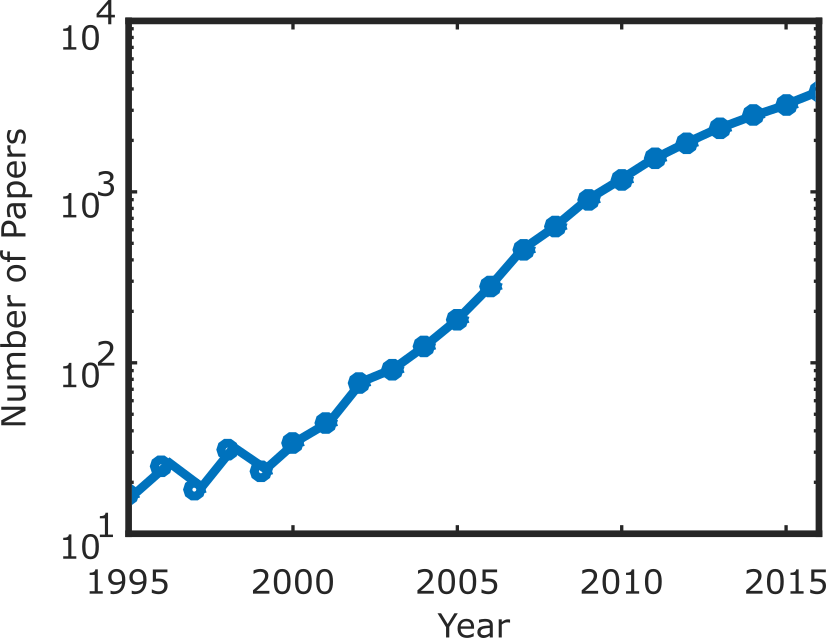
\includegraphics[width=0.40\textwidth]{Chapters/01_Introduction/Figures/paper_PT_therapy.png}
 \caption{Number of papers published containing the terms Plasmonic Photo
 Thermal Therapy since 1995. Note the logarithmic scale in the y-axis.}
 \label{fig:PPTT}
\end{figure}

During the past two decades there has been an increasing interest in gold
nanoparticles as possible agents for medical
treatments\cite{Gobin2007,Huang2006,Huo2014}. The strong interaction between
particles and light makes them ideal candidates not only for labelling but also
for releasing heat into very localized environments
\cite{Huang2008,Huang2006,Gobin2007,Hirsch2003}.
This simple approach can be used for instance to induce death of cancer cells
and is normally referred to as Plasmonic Photo Thermal Therapy (PPTT or PTT
depending on the author). Figure \ref{fig:PPTT} shows the number of papers
published in this field since $1995$. The more-than-exponential increase serves
as a measure for the relevance this technique is gaining.

After decades of research there is however almost no information regarding the
temperatures that need to be reached by the nanoparticles to induce cell death.
Much less is available at a single-particle/single-cell level. Moreover the
field of thermometry at the nanoscale is subject to a heated
debate\cite{Yang2011a,Suzuki2015} since some experimental
findings\cite{Yang2011a} contradict expected values from thermodynamic
considerations\cite{Sato2014}.

Chapter \ref{ch:AntiStokes} of this thesis focuses into the characterization of
the mechanisms that give rise to anti-Stokes luminescence. Discarding
multi-photon processes, photons with higher energies than the excitation energy
require interactions with thermal baths. In a nanoparticle electron and holes
can interact with phonons before recombining radiatively, as discussed in
section \ref{sec:luminescence}.

By carefully fitting the luminescence spectra of single gold nanorods and
nanospheres with a function similar to equation \ref{eqn:antiStokes} it is
possible to extract the surface temperature of the particles. The method
presented in chapter \ref{ch:AntiStokes} does not depend on any ad-hoc
calibration and can be performed in any confocal microscope with a coupled
spectrometer. The chapter shows the increase in temperature with increasing
laser powers and also shows the changes that the luminescence spectra undergo
when increasing the medium's temperature.

The calibration-free procedure is a major improvement over previous techniques
in the field of nano-thermometry. The results from the chapter can have a
significant impact on an emerging community that addresses one of the most
pressing health issues of this time.

\subsection{Plasmon damping as a function of temperature}
Luminescence is not the only method for detecting gold nanorods with an optical
microscope. Gold nanoparticles have a large scattering cross section coinciding
with the plasmon resonance. Exciting nanoparticles with white light allows to
record the scattering spectra in any confocal microscope coupled to a
spectrometer. Since the resonance itself is affected by the surrounding
conditions\cite{Liu2009b,Konrad2013}, it is possible for example to use it for
studying changes in the refractive index of the medium. However the plasmon
resonance energy is not the only interesting property of the nanoparticles; the
plasmon damping rate can also be used to detect changes in the surrounding
conditions.

\begin{sloppypar}

In principle there are four main mechanisms responsible for damping of the
plasmons\cite{Sonnichsen2002,Novo2006,Hu2008}: electron-phonon coupling,
electron-surface interactions, electron-electron collisions and radiative
damping. Out of those only the coupling with phonons shows an appreciable
dependence on temperature\cite{Liu2009b,Konrad2013}. Therefore studying the
dependence of the plasmon width with temperature could lead to an alternative
approach to measure temperature changes.
\end{sloppypar}


Chapter \ref{ch:Damping} focuses on the characterization of the plasmon
resonance of single gold nanorods at various temperatures. The plasmon width
increases linearly with temperature, as predicted from the Debye model of
phonons. Measuring the broadening of the resonance can then be related to
changes in temperature of the surrounding medium. 

The scattering of gold nanorods is much more efficient than their luminescence,
not only because of their large scattering cross section but also because of the
low quantum yield of their emission. Therefore the powers needed for recording
scattering spectra are much lower than the ones employed when exciting the
luminescence of the particles. These lower powers allow to study the plasmon
resonance without inducing a significative increase of temperature. However the
broad distribution of widths and broadening rates found in the studies of
chapter \ref{ch:Damping} does not allow to perform an absolute temperature
measurement but only to measure a relative change. This is similar to other
experiments performed with quantum dots\cite{Yang2011a} and therefore expands
the toolbox of available techniques for thermometry at the nanoscale.

\section{One program to rule them all}
All modern laboratories rely on computer equipment to perform measurements,
ranging from integrated micro controllers to powerful computers. A micro
controller, for example, is responsible for maintaining a stable temperature of
a heating plate; a fast computer on the other hand can analyze data online in high
throughput experiments and take decisions on the fly. Experiments performed at
CERN and in other particle physics accelerators heavily rely on computers to
discard millions of non interesting events and save the relevant ones. However, 
for the average experimentalist there is a big gap between what is needed and
what is available.

Flexible, open source programs to control experiments are hard to find in the
Internet if they exist at all. The absence of a solution generates a double
negative effect: researches find themselves reinventing the wheel more often
than desired and experiments are based on what can be done and not on what is
desired to be done. For example, a simple home built confocal microscope
requires a dedicated computer program to run but it can take months to develop.
Commercial software normally lacks the flexibility that new science needs,
limiting the creativity of researches while planning experiments.

All the chapters of this thesis relied on a flexible computer program that
allowed to plan complex experiments building on software rather than being
limited by it. The program has been made open source and can be found on
Github\footnote{https://github.com/aquilesC/SmartScan}. It started to be
developed for simplifying repetitive tasks as refocusing on a particle or
triggering a spectrometer. Later it evolved into a fully functional graphical
user interface (GUI) for performing and visualizing $2$D and $3$D scans,
acquiring fast timetraces, monitoring an optical tweezer and communicating with
serial devices as well as over the network. The latest developments of the
software allow to define an application programming interface (API) for easy
integration with applications on smartphones or to control several independent
setups through the network (including through the Internet).

Chapter \ref{ch:KCN} shows results where several particles were analyzed while
being etched with potassium cyanide. Studying several nanoparticles under the
same conditions is crucial for characterizing the dependence with the plasmon
resonance and to discard any systematic error. Refocusing on the particles by
hand is too slow for processes that happen as fast as the ones shown in the
chapter and therefore the results shown couldn't have been possible without a
specialized computer program. 

Chapter \ref{ch:Imaging} shows the scanning capabilities of the software for
imaging purposes. Moreover the specific program for acquiring the power
dependence plots can be written in about $20$ lines of code. When varying the
temperature of the sample as in chapters \ref{ch:AntiStokes} and
\ref{ch:Damping} being able to refocus on a reference particle to compensate for
the drift of the setup was of utmost importance.

The software even if developed with an optical microscope in mind, can be easily
extended to other configurations. Choosing Python as the programming language
provides platform independence; it can run without inconvenience on several
Windows versions, Mac OS and Linux. The main objective of the program is to
provide a lower level layer on which to build creative solutions to complex
problems.

\references{Chapters/01_Introduction/introduction}